%%%%%%%%%%%%%%%%%%%%%%%%%%%%%%%%%%%%%%%%%%%%%%%%%%%%%%%%%%%%%%%%%%%%%%%
%%%%%%%%%%%%%%%%%%%%%%%%%%%%%%%%%%%%%%%%%%%%%%%%%%%%%%%%%%%%%%%%%%%%%%% 
%%%%%%%%%%%       								 Preamble				         	                                                        %%%%%%%%%% 
%%%%%%%%%%%%%%%%%%%%%%%%%%%%%%%%%%%%%%%%%%%%%%%%%%%%%%%%%%%%%%%%%%%%%%% 
%%%%%%%%%%%%%%%%%%%%%%%%%%%%%%%%%%%%%%%%%%%%%%%%%%%%%%%%%%%%%%%%%%%%%%% 
\documentclass[10pt]{beamer}
\usepackage{setspace}
\usepackage{color}
\usepackage{amsmath,lmodern}
\usepackage{hyperref}
\usepackage{graphicx}
\usepackage{multirow}
\usepackage{tikz}
\usetikzlibrary{fit,shapes.misc}
\usepackage{pdflscape}
\usepackage{amsmath}
\usepackage{lscape}
\usepackage{multirow}
\usepackage{enumerate}
\usepackage{mathtools}
\usepackage{epstopdf}
\usepackage{pdfpages}
\usepackage{bm}
\usepackage{appendixnumberbeamer}
\usepackage{color,soul}
\usepackage{grffile}
\usepackage{float}
\usepackage{relsize}
\usepackage{tcolorbox}
\newcounter{nodemarkers}
\usepackage{tikz}
\newcommand{\toplinesmall}{%
  \tikz[remember picture,overlay] {%
    \draw[blue,thick] ([yshift=-1cm, xshift=.9cm]current page.north west)
             -- ([yshift=-1cm,xshift=3.6cm]current page.north west);}}
             
\newcommand{\toplinemedium}{%
  \tikz[remember picture,overlay] {%
    \draw[blue,thick] ([yshift=-1cm, xshift=.9cm]current page.north west)
             -- ([yshift=-1cm,xshift=6.2cm]current page.north west);}}
 
 \newcommand{\toplinelarge}{%
  \tikz[remember picture,overlay] {%
    \draw[blue,thick] ([yshift=-1cm, xshift=.9cm]current page.north west)
             -- ([yshift=-1cm,xshift=8.9cm]current page.north west);}}           
             
 \newcommand{\toplinexlarge}{%
  \tikz[remember picture,overlay] {%
    \draw[blue,thick] ([yshift=-1cm, xshift=.9cm]current page.north west)
             -- ([yshift=-1cm,xshift=12cm]current page.north west);}}                       
             
\setbeamertemplate{footline}
{
  \leavevmode%
  \hbox{%
  \begin{beamercolorbox}[wd=.333333\paperwidth,ht=2.25ex,dp=1ex,center]{author in head/foot}%
    \usebeamerfont{author in head/foot}{\textcolor{blue}{ECON712}}
  \end{beamercolorbox}%
  \begin{beamercolorbox}[wd=.333333\paperwidth,ht=2.25ex,dp=1ex,center]{title in head/foot}%
    \usebeamerfont{title in head/foot}{\textcolor{blue}{Winter 2026}}
  \end{beamercolorbox}%
  \begin{beamercolorbox}[wd=.333333\paperwidth,ht=2.25ex,dp=1ex,right]{date in head/foot}%
    \usebeamerfont{date in head/foot}{\textcolor{blue}{Lecture 12  \: \: \: \: \: \: \: }
    \insertframenumber{} / \inserttotalframenumber\hspace*{2ex}} 
  \end{beamercolorbox}}%
  \vskip0pt%
}
\newtheorem{proposition}[theorem]{Proposition}

\newcommand\marktopleft[1]{%
    \tikz[overlay,remember picture] 
        \node (marker-#1-a) at (-0.2,1.2ex) {};%
}
\newcommand\markbottomright[1]{%
    \tikz[overlay,remember picture] 
        \node (marker-#1-b) at (0.16,-1ex) {};%
    \tikz[overlay,remember picture,thick,inner sep=4pt]
        \node[draw,rectangle,rounded corners, blue, fit=(marker-#1-a.center) (marker-#1-b.center)] {};%
}

\setbeamertemplate{caption}{\raggedright\insertcaption\par}
\setbeamertemplate{itemize items}[ball]
\setbeamertemplate{itemize subitem}[triangle]
\setbeamertemplate{itemize subsubitem}[triangle]
\tcbset{colframe=white,colback=white,nobeforeafter}
\beamertemplatenavigationsymbolsempty
\addtobeamertemplate{frametitle}{\vspace*{0.19cm}}{\vspace*{0cm}}


%%%%%%%%%%%%%%%%%%%%%%%%%%%%%%%%%%%%%%%%%%%%%%%%%%%%%%%%%%%%%%%%%%%%%%%
%%%%%%%%%%%%%%%%%%%%%%%%%%%%%%%%%%%%%%%%%%%%%%%%%%%%%%%%%%%%%%%%%%%%%%% 
%%%%%%%%%  									    Define Title									                                       %%%%%%%%%
%%%%%%%%%%%%%%%%%%%%%%%%%%%%%%%%%%%%%%%%%%%%%%%%%%%%%%%%%%%%%%%%%%%%%%%
%%%%%%%%%%%%%%%%%%%%%%%%%%%%%%%%%%%%%%%%%%%%%%%%%%%%%%%%%%%%%%%%%%%%%%% 
\title{ECON 712: Applied Econometrics} 
\author{Lecture 12: Statistical Properties of OLS, part II}
\date{}
\AtBeginSection[]
{
 \begin{frame}<beamer>
 \tableofcontents[currentsection]
 \end{frame}
}
%%%%%%%%%%%%%%%%%%%%%%%%%%%%%%%%%%%%%%%%%%%%%%%%%%%%%%%%%%%%%%%%%%%%%%%
%%%%%%%%%%%%%%%%%%%%%%%%%%%%%%%%%%%%%%%%%%%%%%%%%%%%%%%%%%%%%%%%%%%%%%% 
%%%%%%%% 						     				Document								                                                %%%%%%%%
%%%%%%%%%%%%%%%%%%%%%%%%%%%%%%%%%%%%%%%%%%%%%%%%%%%%%%%%%%%%%%%%%%%%%%%
%%%%%%%%%%%%%%%%%%%%%%%%%%%%%%%%%%%%%%%%%%%%%%%%%%%%%%%%%%%%%%%%%%%%%%% 
\begin{document}
\setbeamercovered{transparent}

\begin{frame}
\maketitle
\end{frame}

\begin{frame}
\frametitle{\: \: \: Unbiasedness} 
\toplinemedium
\begin{itemize}
\item Under strict exogeneity, $\mathbb{E}[\bm{u}|\bm{X}]=\bm{0}$, OLS/MM is unbiased:
\begin{eqnarray*}
\begin{array}{rl}
\bm{\hat{\beta}}^{ols}&=(\bm{X}^T \bm{X})^{-1} \bm{X}^T \bm{y} \\[1.2ex]
 \bm{\hat{\beta}}^{ols}  &=\bm{\beta}+(\bm{X}^T \bm{X})^{-1} \bm{X}^T \bm{u}  \\[1.2ex]
                                 \mathbb{E}[\bm{\hat{\beta}}^{ols}|\bm{X}] &=\bm{\beta}\underbrace{=}_{\text{by LIE}}  \mathbb{E}[\bm{\hat{\beta}}^{ols}]
\end{array}
\end{eqnarray*}
\item Pre-determinedness, $\mathbb{E}[u_i|x_{1i}, \cdot , x_{ki}]=0$, is not enough
\vspace{0.11in}
\item The linear CEF has to be correctly specified
\end{itemize}
\end{frame}


\begin{frame}
\frametitle{\: \: \: Variance under Spherical Errors} 
\toplinelarge
\begin{itemize}
\item Another important property of OLS is the conditional \textcolor{blue}{variance-covariance} matrix of estimates:
\begin{eqnarray*}
Var[\bm{\hat{\beta}}^{ols}|\bm{X}]=\mathbb{E}\left[(\bm{\hat{\beta}}^{ols}-\bm{\beta})(\bm{\hat{\beta}}^{ols}-\bm{\beta})^T \mathbb{|} \bm{X}\right]
\end{eqnarray*}
\item Assume that $\mathbb{E}\left[\bm{u}\bm{u}^T \mathbb{|} \bm{X}\right]=\sigma^2 \: \bm{I}$, then 
\begin{eqnarray*}
Var[\bm{\hat{\beta}}^{ols}|\bm{X}]=\sigma^2 (\bm{X}^T\bm{X})^{-1}
\end{eqnarray*}
\begin{itemize}
\item In practice, we estimate $\sigma^2$ by $\hat{\sigma}^2=\bm{\hat{u}}^T\bm{\hat{u}}(n-k)^{-1}$ 
\end{itemize}
\vspace{0.11in}
\item Spherical error terms is a very strict assumption, which is not usually satisfied, specially if the CEF is not linear
\vspace{0.11in}
\item  By the law of total variance, the unconditional variance is 
\begin{eqnarray*}
Var(\bm{\hat{\beta}}^{ols})=\sigma^2 \mathbb{E}[(\bm{X}^T\bm{X})^{-1}]
\end{eqnarray*}
\end{itemize}
\end{frame}



\begin{frame}
\frametitle{\: \: \: Distribution of regressors under Gauss-Markov} 
\toplinexlarge
\begin{itemize}
\item Classical or Gauss Markov Assumptions of Multiple Regression are:
\begin{enumerate}
\item If the population equation is given by (linear CEF) 
\begin{eqnarray*}
\bm{y}=\bm{X} \bm{\beta}+\bm{u}
\end{eqnarray*}
\item No perfect multicollinearity (i.e. $\bm{X}$ has full rank)
\item Zero Conditional Mean (i.e. $E[\bm{u}|\bm{X}]=\bm{0}$)
\item Homoskedasticity and no serial correlation (i.e. $Var[\bm{u}|\bm{X}]=\sigma^2 \: \bm{I}_{n}$)
\item Population conditional error terms are jointly Normal: $\bm{u}|\bm{X}\sim N\left[\bm{0},\sigma^2 \: \bm{I}_N\right]$
\end{enumerate}
\item This yield the following result:
\begin{eqnarray*}
\bm{\hat{\beta}}|\bm{X}\sim N\left[\bm{\beta},\sigma^2 \: (\bm{X}^T\bm{X})^{-1}\right]
\end{eqnarray*}
\item Because of properties of the multivariate normal distribution:
\begin{eqnarray*}
\hat{\beta}_j|\bm{X}\sim N\left[\beta_j,\sigma^2 \: (\bm{X}^T\bm{X})_{jj}^{-1}\right]
\end{eqnarray*}
\item We can write the variance of the estimator in multiple regression as  
\begin{eqnarray*}
Var[\hat{\beta_j}|\bm{X}]=\frac{\sigma^2}{SST_j (1-R^2_{j})}
\end{eqnarray*}
\end{itemize}
\end{frame}


\begin{frame}
\frametitle{\: \: \: Consistency} 
\toplinesmall
\begin{itemize}
\item Classical Assumptions are very restrictive and not usually satisfied in practice
\vspace{0.11in}
\item  Therefore, modern econometrics relies on asymptotic properties of estimators, which are satisfied under weaker conditions 
\vspace{0.11in}
\item For instance, if we assume that $\mathbb{E}[\bm{X}_i \: u_i]=\bm{0}$, then
\begin{eqnarray*}
\begin{array}{ll}
\underset{n\rightarrow \infty}{plim} \bm{\hat{\beta}}^{ols}  &=\underset{n\rightarrow \infty}{plim}\left[\bm{\beta}+(\frac{1}{n}\bm{X}^T \bm{X})^{-1} (\frac{1}{n}\bm{X}^T \bm{u}) \right] \\[1.4ex]
														         &=\bm{\beta}+ (\bm{S_{X^TX}})^{-1} \underset{n\rightarrow \infty}{plim}  (\frac{1}{n}\bm{X}^T \bm{u}) \\[1.4ex]
															&=\bm{\beta} \text{   (the OLS estimator is consistent)}
\end{array}
\end{eqnarray*}
\item Because we do not need mean independence, but zero covariance, the CEF does not need to be linear 
\vspace{0.11in}
\item Pre-determinedness is enough
\end{itemize}
\end{frame} 

\begin{frame}
\frametitle{\: \: \: Asymptotic Distribution of OLS}
\toplinelarge
\begin{itemize}

\item OLS decomposition:
\[
\sqrt{n}(\hat{\bm{\beta}}^{ols}-\bm{\beta})
=
\left(\frac{1}{n}\bm{X}^T\bm{X}\right)^{-1}
\sqrt{n}\left(\frac{1}{n}\bm{X}^T\bm{u}\right)
\]

\item Under \textcolor{blue}{iid} errors and $\mathbb{E}[X_i u_i]=0$:
\[
\frac{1}{n}\bm{X}^T\bm{X}
\xrightarrow{p}
S_{X^{\top}X}
\quad\text{(LLN)}
\]

\[
\sqrt{n}\left(\frac{1}{n}\bm{X}^T\bm{u}\right)
\xrightarrow{d}
N(\bm{0},\underbrace{
\mathbb{E}\!\left[(X_i u_i)(X_i u_i)^{\top}\right]}_{=\Omega})
\quad\text{(MCLT)}
\]

\item By Slutsky:
\[
\sqrt{n}(\hat{\bm{\beta}}^{ols}-\bm{\beta})
\xrightarrow{d}
N\!\left(
\bm{0},
S_{X^{\top}X}^{-1}
\Omega
S_{X^{\top}X}^{-1}
\right)
\]

\end{itemize}
\end{frame}

\begin{frame}
\frametitle{\: \: \: Asymptotic Variance of OLS}
\toplinelarge
\begin{itemize}
\item We can write the matrix $\Omega$ as follows:
\begin{eqnarray*}
\Omega=\mathbb{E}\!\left[(\bm{X_i} u_i u_i)^{T} \bm{X_i}^T\right]=\mathbb{E}\!\left[u_i^2 \bm{X_i} \bm{X_i}^T\right]
\end{eqnarray*}
\begin{itemize}
\item If $\mathbb{E}\!\left[u_i^2 | \bm{X_i}\right]=\sigma^2$, then by LIE
\begin{eqnarray*}
\begin{array}{l}
\mathbb{E}\!\left[u_i^2 \bm{X_i} \bm{X_i}^T\right]=\mathbb{E}\!\left[\mathbb{E}\! \left[u_i^2 |\bm{X_i}\right] \bm{X_i} \bm{X_i}^T\right] \\[1.2ex]
\mathbb{E}\!\left[u_i^2 \bm{X_i} \bm{X_i}^T\right]=\sigma^2 S_{X^{\top}X}
\end{array}
\end{eqnarray*}
\item This is the same variance as in the finite sample case, but with a large sample, we can set $S_{X^{\top}X}=(\bm{X}^T \bm{X})$ 
\vspace{0.11in} 
\item Then,
\begin{eqnarray*}
\sqrt{n}(\hat{\bm{\beta}}^{ols}-\bm{\beta})\xrightarrow{d} N(\bm{0}, n \: \sigma^2(\bm{X}^T \bm{X})^{-1})
\end{eqnarray*}
\end{itemize}
\end{itemize}
\end{frame}


\begin{frame}
\frametitle{\: \: \: Heteroscedasticity-Robust Variance}
\toplinelarge
\begin{itemize}
\item Sometimes, error terms are non-spherical:
\begin{eqnarray*}
E[\bm{u}\bm{u}'|\bm{X}]=\bm{\Sigma_u} \neq \sigma^2 \: I_N
\end{eqnarray*}
\item For instance, when there is heteroscedasticity
\begin{columns}
\begin{column}{0.4\linewidth}
\begin{eqnarray*}
\bm{\Sigma_u}=
 \begin{bmatrix}
    \sigma^2_1 & 0  & \cdots &0        \\
     0           & \sigma^2_2  & \cdots &0 \\
     \vdots  &\vdots           &\vdots &\vdots \\ 
      0           & 0  & \cdots &  \sigma^2_N  \\
\end{bmatrix}
\end{eqnarray*}
\end{column}
\begin{column}{0.7\linewidth}
\centering
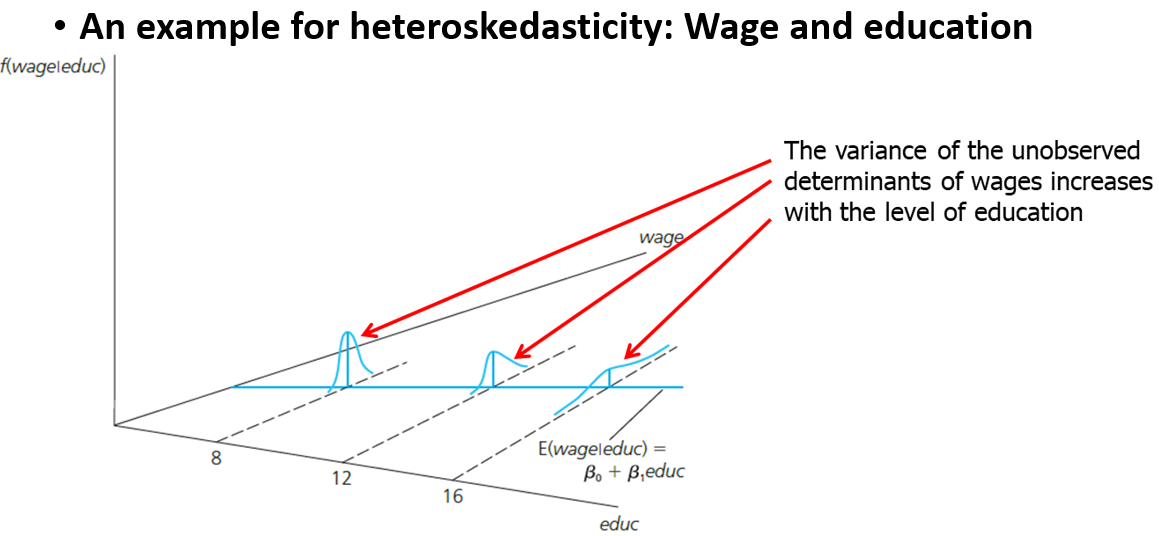
\includegraphics[scale=.24]{hetero}
\end{column}
\end{columns}
\end{itemize}
\end{frame}

\begin{frame}
\frametitle{\: \: \: Heteroscedasticity Robust Variance}
\toplinelarge
\begin{itemize}
\item In this case, the Variance-Covariance Matrix estimated in a previous slide is incorrect:
\begin{eqnarray*}
Var[\bm{\hat{\beta}}|\bm{X}]=(\bm{X}'\bm{X})^{-1} \: \bm{X}' \: \bm{\Sigma_u} \bm{X} (\bm{X}' \bm{X})^{-1}
\end{eqnarray*}
\item We could estimate $\bm{\Sigma_u}$ as follows:
\begin{eqnarray*}
\bm{\hat{\Sigma}_u}=
 \begin{bmatrix}
    \hat{u}^2_1 & 0  & \cdots &0        \\
     0           & \hat{u}^2_2  & \cdots &0 \\
     \vdots  &\vdots           &\vdots &\vdots \\ 
      0           & 0  & \cdots &  \hat{u}^2_n  \\
\end{bmatrix}
\end{eqnarray*}
\item \textcolor{blue}{HOWEVER}, this is not a consistent estimator as the number of parameters increases with $n$
\end{itemize}
\end{frame}

\begin{frame}
\frametitle{\: \: \: Heteroscedasticity-Robust Variance}
\toplinelarge
\begin{itemize}
\item We instead estimate the following term:
\begin{eqnarray*}
\bm{X}' \: \bm{\hat{\Sigma}_u} \bm{X}
\end{eqnarray*}
\begin{itemize}
\item This is a $kxk$ matrix called a sandwich covariance matrix
\vspace{.11in}
\item An element of the previous matrix is: $\mathlarger{\sum}_{i=1}^{n}\hat{u}^2_i \: x_{is} \: x_{ij}$
\vspace{.11in}
\item It can be shown that, under certain conditions, this is a consistent estimate (it biased in small samples as $E[\hat{u}^2_i|\bm{X}]\neq \sigma^2_i$
\end{itemize}
\vspace{.11in}
\item In this case, the OLS estimator is not the most efficient estimator (FGLS is), but it is still used in practice
\end{itemize}
\end{frame}

\begin{frame}
\frametitle{\: \: \: Cluster Robust Variance }
\toplinelarge
\begin{itemize}
\item Suppose there is a natural grouping of data:
\begin{eqnarray*}
y_{ig}=\bm{x}_{ig} \: \bm{\beta} +u_{ig} 
\end{eqnarray*}
or
\begin{eqnarray*}
\begin{array}{ll}
\bm{y}_{g}=\bm{X}_{g} \: \bm{\beta} +\bm{u}_{g}  & \text{  for } g=1,\cdots,G
\end{array} 
\end{eqnarray*}
where 
\begin{eqnarray*}
 \bm{X}_g=\begin{bmatrix}
    1 & x_{12} & x_{13} & \cdots & x_{1k} \\
    1 & x_{22} & x_{23} & \cdots & x_{2k} \\
     \vdots    &   \vdots      &  \vdots &  \vdots  &\vdots          \\
    1 & x_{n_g2} & x_{n_g3} & \cdots & x_{n_gk} \\
  \end{bmatrix}
\end{eqnarray*}
\item The total number of observations is: $n=\mathlarger{\sum}_{g=1}^{G} n_g$
\end{itemize}
\end{frame}

\begin{frame}
\frametitle{\: \: \: Cluster Robust Variance }
\toplinelarge
\begin{itemize}
\item In addition, suppose that the variance structure of the error term is:
\begin{eqnarray*}
E[\bm{u}_g \: \bm{u}'_g]=
\bm{\Sigma}_g=
 \begin{bmatrix}
    \sigma^2 &   \sigma_{1,2}& \cdots &\sigma_{1,n_g}        \\
     \sigma_{1,2}           & \sigma^2  & \cdots &\sigma_{2,n_g} \\
     \vdots  &\vdots           &\vdots &\vdots \\ 
      \sigma_{1,n_g}            & \sigma_{2,n_g}    & \cdots &  \sigma^2  \\
\end{bmatrix}
\end{eqnarray*}
and 
\begin{eqnarray*}
E[\bm{u} \: \bm{u}']=
\bm{\Sigma_u}=
 \begin{bmatrix}
    \bm{\Sigma}_1 &   \bm{0}& \cdots &\bm{0}        \\
     \bm{0}          & \bm{\Sigma}_2 & \cdots &\bm{0} \\
     \vdots  &\vdots           &\vdots &\vdots \\ 
      \bm{0}            & \bm{0}    & \cdots &  \bm{\Sigma}_G  \\
\end{bmatrix}
\end{eqnarray*}
\end{itemize}
\end{frame}

\begin{frame}
\frametitle{\: \: \: Cluster Robust Variance } 
\toplinelarge
\begin{itemize}
\item In this case the sandwich estimator has the following form:
\begin{eqnarray*}
\bm{X'}\bm{\hat{\Sigma}_u}\bm{X}=\mathlarger{\sum}_{g=1}^{G} \bm{X'}_g \bm{\hat{u}}_g \bm{\hat{u}'}_g \bm{X}_g
\end{eqnarray*}
\item Asymptotic Theory in this case applies for $G\rightarrow \infty$
\begin{itemize}
\vspace{0.11in}
\item A small number of groups result in large and very biased Se, independently of the size of $n_g$, specially when observations within groups are highly correlated
\end{itemize}
\vspace{0.11in}
\item It is always important to cluster if you suspect within group correlation, however, Clustering Se is extremely important in the following cases:
\begin{itemize}
\vspace{0.11in}
\item Time Series data with autocorrelated errors: $y_{it}=\bm{X}_{it} \bm{\beta}+u_{it}$
\vspace{0.11in}
\item Treatment level is higher than individual observations: $y_{i}=\bm{X}_{g} \bm{\beta}+u_{i}$
\end{itemize}
\end{itemize}
\end{frame}



\end{document}
